\setbeamercolor{background canvas}{bg=fitblue}
\begin{frame}
  \frametitle{Procedural generation / Procedurální generování}
  \begin{center}
    \Huge {\color{white}Procedural generation / Procedurální generování}
  \end{center}
\end{frame}
\setbeamercolor{background canvas}{bg=white}

\begin{frame}\frametitle{Procedurální generování}\scriptsize
\begin{itemize}
  \item We do not have to store data of objects (vertices, textures, ...).
  \item We only stores templates and algorithms how to generate objects.
  \item Algorithm memory footprint is only few kB.
  \item Parameters can be stored in text files.
  \item Even template can be generated.
  \item Small memory footprint versus time to generate object.
\end{itemize}
\begin{itemize}
  \item{Neukládáme data grafických objektů.}
  \item{Neukládáme vrcholy, pixely, barvy, ...}
  \item{Ukládáme šablony a způsob vygenerování grafického objektu.}
  \item{Uložení algoritmu pro vygenerování zabírá pár kB.}
  \item{Uložení v textovém souboru - parametry.}
  \item{Můžeme generovat i šablony.}
  \item{Málo místa pro uložení vs doba generování.}
\end{itemize}
\end{frame}

\begin{frame}\frametitle{Fractals / Fraktály}
	\begin{figure}[h]
		\includegraphics[width=10cm,keepaspectratio]{pics/procedural/fractal.jpg}
	\end{figure}
\end{frame}

\begin{frame}\frametitle{Fractals / Fraktály}
	\begin{figure}[h]
		\includegraphics[width=2.8cm,keepaspectratio]{pics/procedural/weed0.jpg}
		\includegraphics[width=2.8cm,keepaspectratio]{pics/procedural/weed1.jpg}
		\includegraphics[width=2.8cm,keepaspectratio]{pics/procedural/weed2.jpg}
		\includegraphics[width=2.8cm,keepaspectratio]{pics/procedural/weed3.jpg}
	\end{figure}
	\url{http://www.dangries.com/Flash/FractalMakerExp/FractalMaker_exp.html}
\end{frame}

\begin{frame}\frametitle{L-systems / L-systém}
	\begin{figure}[h]
		\includegraphics[width=4cm,keepaspectratio]{pics/procedural/lsystem.jpg}
		\includegraphics[width=4cm,keepaspectratio]{pics/procedural/lsystem1.jpg}
	\end{figure}
	\url{http://malsys.cz/}
\end{frame}

\begin{frame}\frametitle{L-systems / L-systém}
	\begin{figure}[h]
		\includegraphics[width=10cm,keepaspectratio]{pics/procedural/castle.jpg}
	\end{figure}
	\url{http://procworld.blogspot.com/}
\end{frame}

\begin{frame}\frametitle{Noise, voronoi diagrams / Šumy a voroného diagramy}
	\begin{itemize}
		\item Perlin/Simple noise
    \item Voronoi diagram / Voroného diagramy
	\end{itemize}
	\begin{figure}[h]
		\includegraphics[width=3cm,keepaspectratio]{pics/procedural/simple_noise}
		\includegraphics[width=3cm,keepaspectratio]{pics/procedural/midpoint_noise}
		\includegraphics[width=3cm,keepaspectratio]{pics/procedural/voronoid}
	\end{figure}
\end{frame}


\begin{frame}\frametitle{Noise based textures / Textury založené na šumech}
	\begin{figure}[h]
		\includegraphics[width=3cm,keepaspectratio]{pics/procedural/tex00.jpg}
		\includegraphics[width=3cm,keepaspectratio]{pics/procedural/tex01.jpg}
		\includegraphics[width=3cm,keepaspectratio]{pics/procedural/tex02.jpg}
	\end{figure}
\end{frame}

\begin{frame}\frametitle{Procedural textures / Procedurální textury}
\begin{columns}[c]
\column{.5\textwidth}
  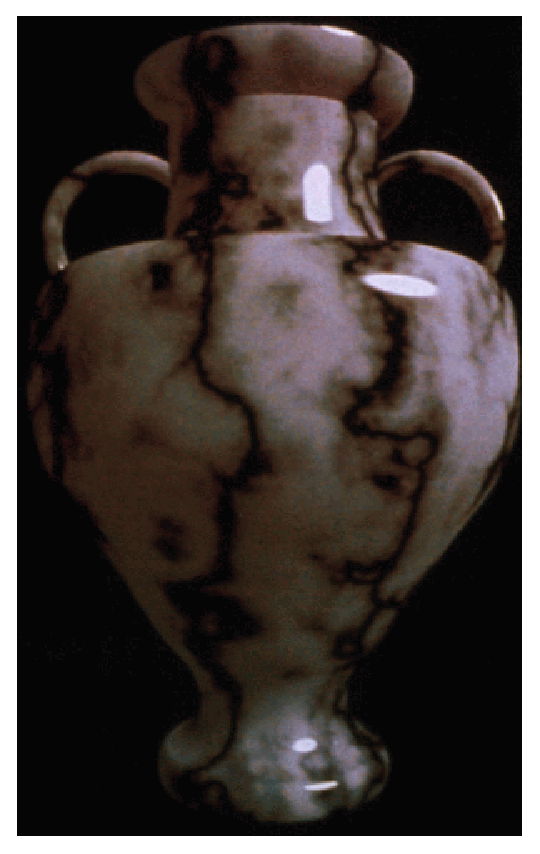
\includegraphics[width=0.7\textwidth]{pics/procedural/vase.eps}
\column{.5\textwidth}
\begin{itemize}
  \item Texture is computed in shader on demand.
  \item Small memory footprint.
  \item Infinite resolution.
  \item Suitable for demos.
  \item Noise.
\end{itemize}
\begin{itemize}
  \item Výpočet hodnoty v shaderu.
  \item Málo paměti.
  \item Neomezené rozlišení.
  \item Vhodné pro dema.
  \item Šum
\end{itemize}
\end{columns}
\end{frame}

\begin{frame}\frametitle{Šum v grafice}
We need noise functions / Chceme šumové funkce
\begin{itemize}
  \item float noise(float p)
  \item float noise(vec2 p)
  \item ...
\end{itemize}
\vfill
\begin{itemize}
   \item Pseudorandom / Pseudonáhodné
   \item Input is in range: / Výstup v: $[0,1]$ / $[-1,1]$
   \item Deterministic / Deterministické
   \item Limited frequency spectrum / Omezené frekvenční spektrum
\end{itemize}
\end{frame}

\begin{frame}[fragile]\frametitle{Value noise / Hodnotový šum}\scriptsize
\begin{columns}[c]
\column{.5\textwidth}
  \begin{itemize}
      \item Randomly generated textures / Náhodně vygenerovaná textura.
      \item The repetition pattern is visible / Rychle se opakuje.
      \item Interpolation and tiling can be performed by OpenGL. / Interpolaci a opakování zařídí OpenGL.
  \end{itemize}
\column{.5\textwidth}
  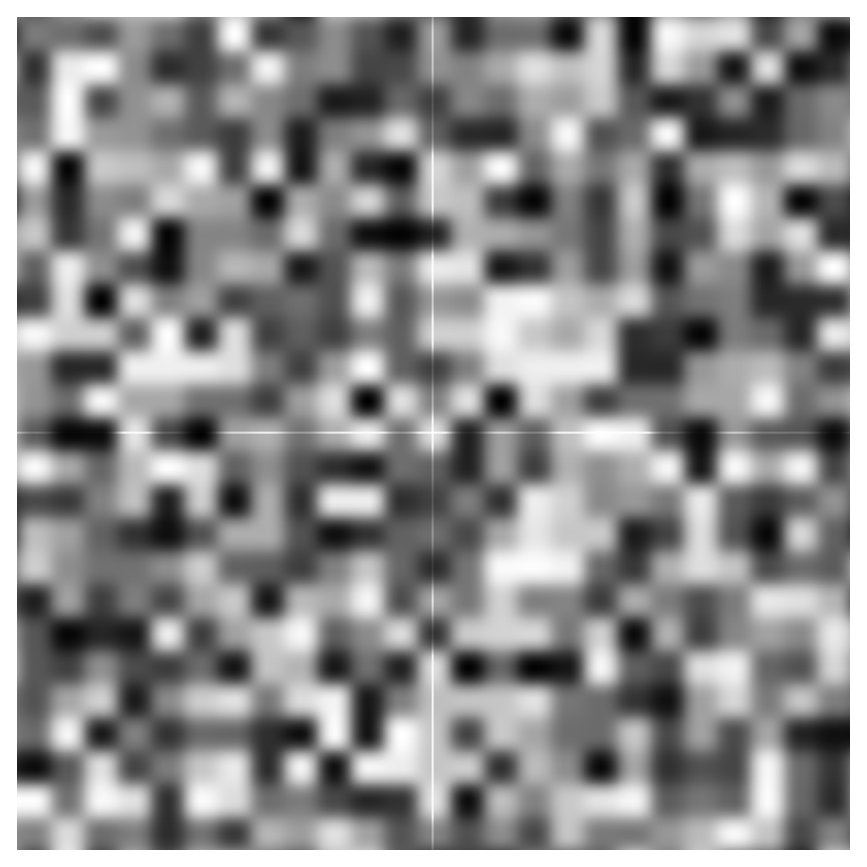
\includegraphics[width=0.5\textwidth]{pics/procedural/value_noise.eps}
\end{columns}

\begin{minted}[bgcolor=bg]{packages/graphics.py:GLShaderLexer -x}
float noise(vec2 p)
{
  return 2*texture(noiseTexture, p).x - 1;
}
\end{minted}
\end{frame}

\begin{frame}[fragile]\frametitle{Gradient noise / Gradientní šum}\scriptsize
\begin{columns}[c]
\column{.5\textwidth}
  \begin{itemize}
      \item Texture stores gradients. / V textuře jsou \textbf{gradienty}.
      \item We need to compute directional vector from texels to samples. / Spočítáme si směrové vektory od \textbf{texelů} ke \textbf{vzorku}.
      \item Scalar multiplication od directions and gradient computes the resoluting noise. / Skalární součin směrů s gradienty dává výsledný šum.
  \end{itemize}
  
\includegraphics[width=.5\textwidth]{pics/procedural/grad_noise.eps}
\column{.5\textwidth}
  
\includegraphics[width=.5\textwidth]{pics/procedural/perlin_noise.eps}
\end{columns}
Perlin K.; Implementing Improved Perlin Noise, GPU Gems\\
Green S.; Implementing Improved Perlin Noise, GPU Gems 2
\end{frame}

\begin{frame}[fragile]\frametitle{Fractal noise / Fraktální šum}
\begin{columns}[c]
\column{.5\textwidth}
  \begin{itemize}
    \item Add layers with different frequencies and amblitudes. / Sčítáme vrstvy o různé frekvenci a amplitudě
    \item Octaves / Oktávy
  \end{itemize}
\column{.5\textwidth}
    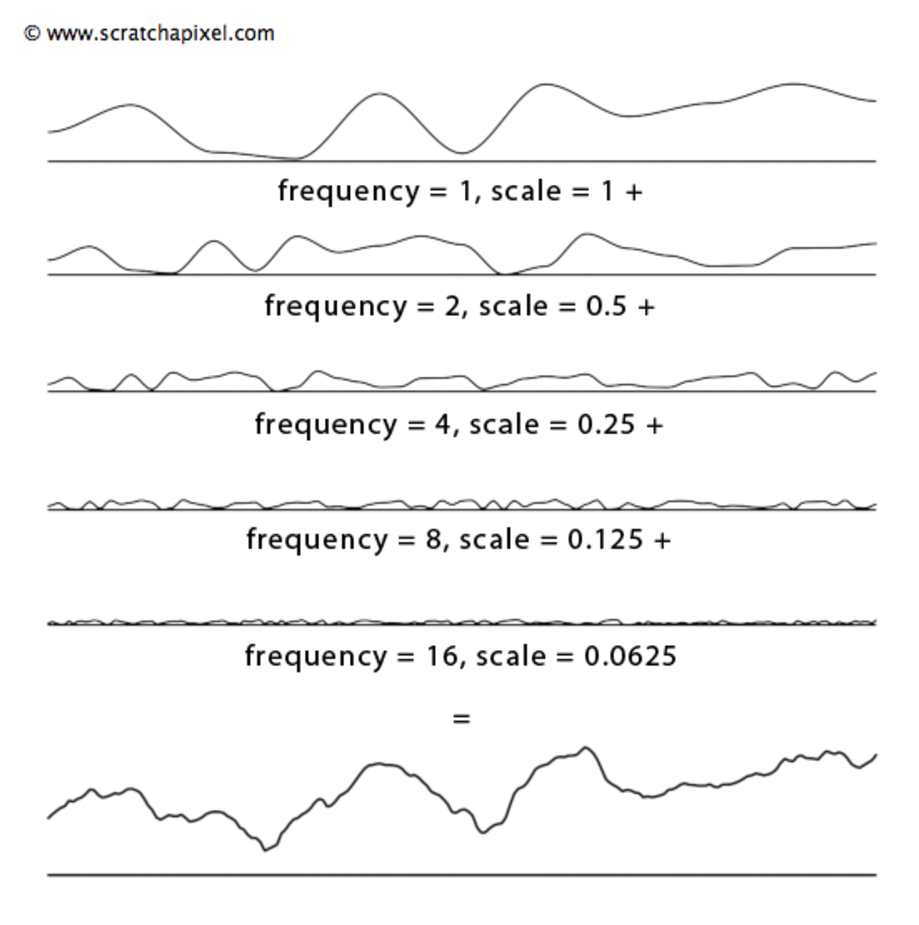
\includegraphics[width=0.5\textwidth]{pics/procedural/1dnoise-fractal.eps}
\end{columns}
\begin{minted}[bgcolor=bg]{packages/graphics.py:GLShaderLexer -x}
float fnoise(vec2 p)
{
  return noise(p)
      + 0.5*noise(2*p)
      + 0.25*noise(4*p);
}
\end{minted}
\end{frame}

\begin{frame}\frametitle{Result / Výsledek}
  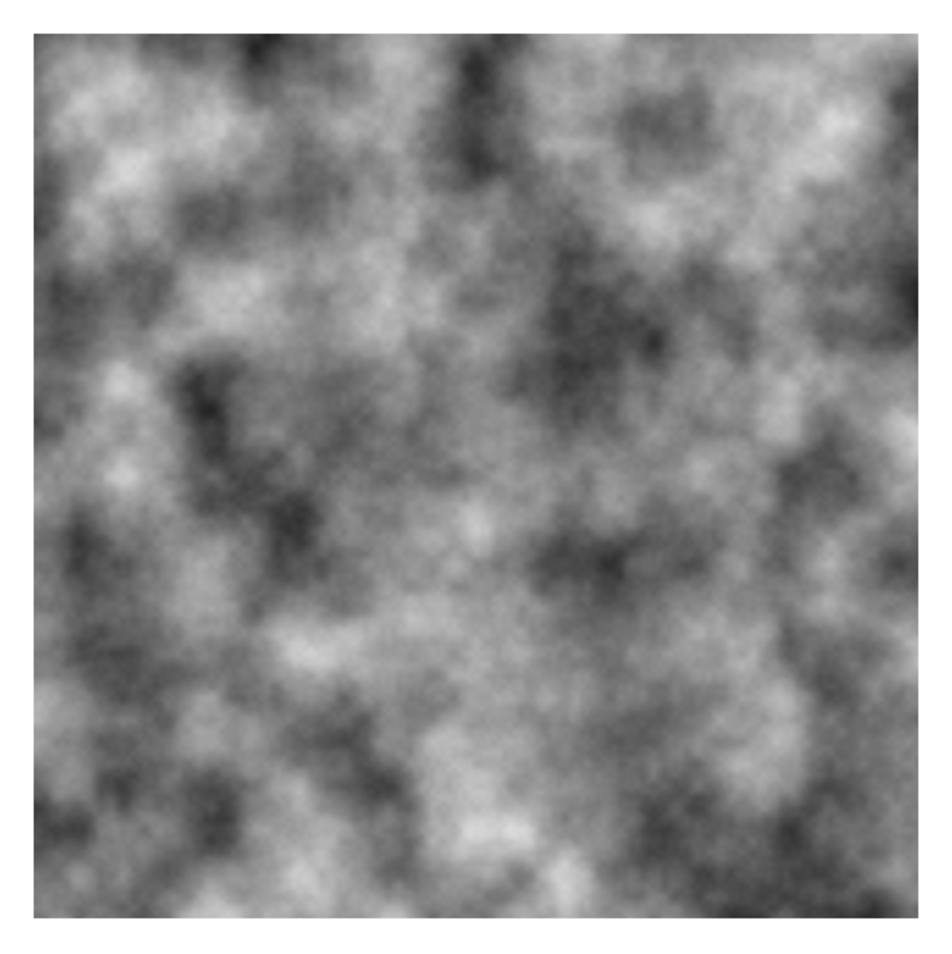
\includegraphics[width=0.7\textwidth]{pics/procedural/2dnoise-fractal.eps}
\end{frame}

\begin{frame}\frametitle{Simple example / Jednoduchý priklad}
  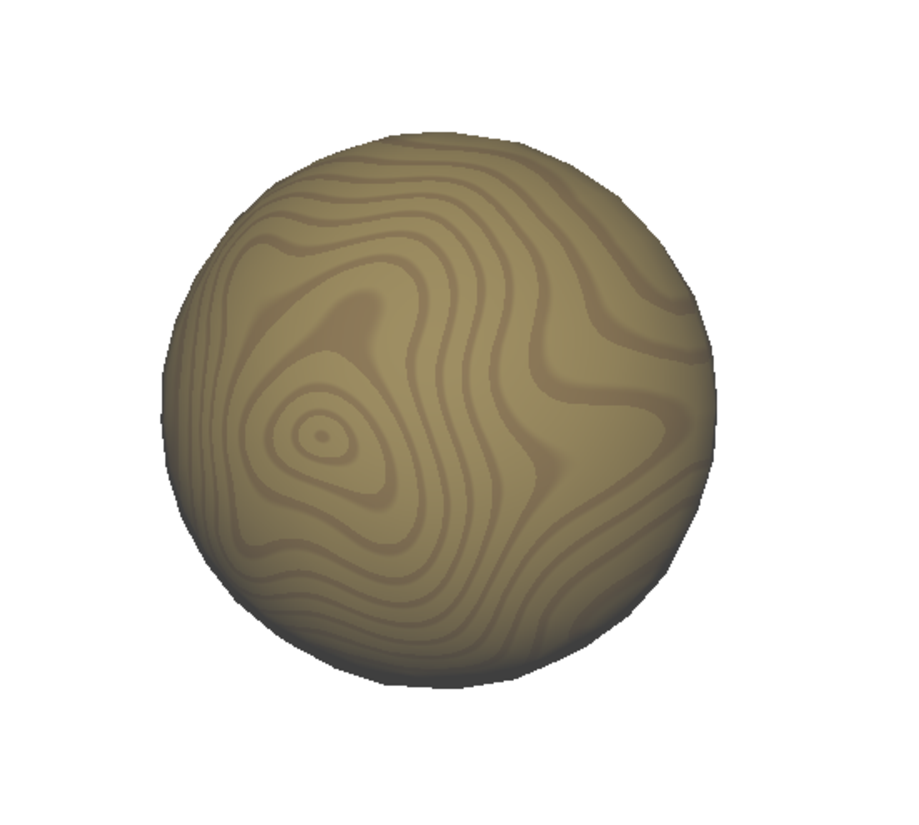
\includegraphics[width=0.5\textwidth]{pics/procedural/drevo.eps}
\end{frame}
 
\begin{frame}[fragile]\frametitle{Annual ring / Letokruhy}
  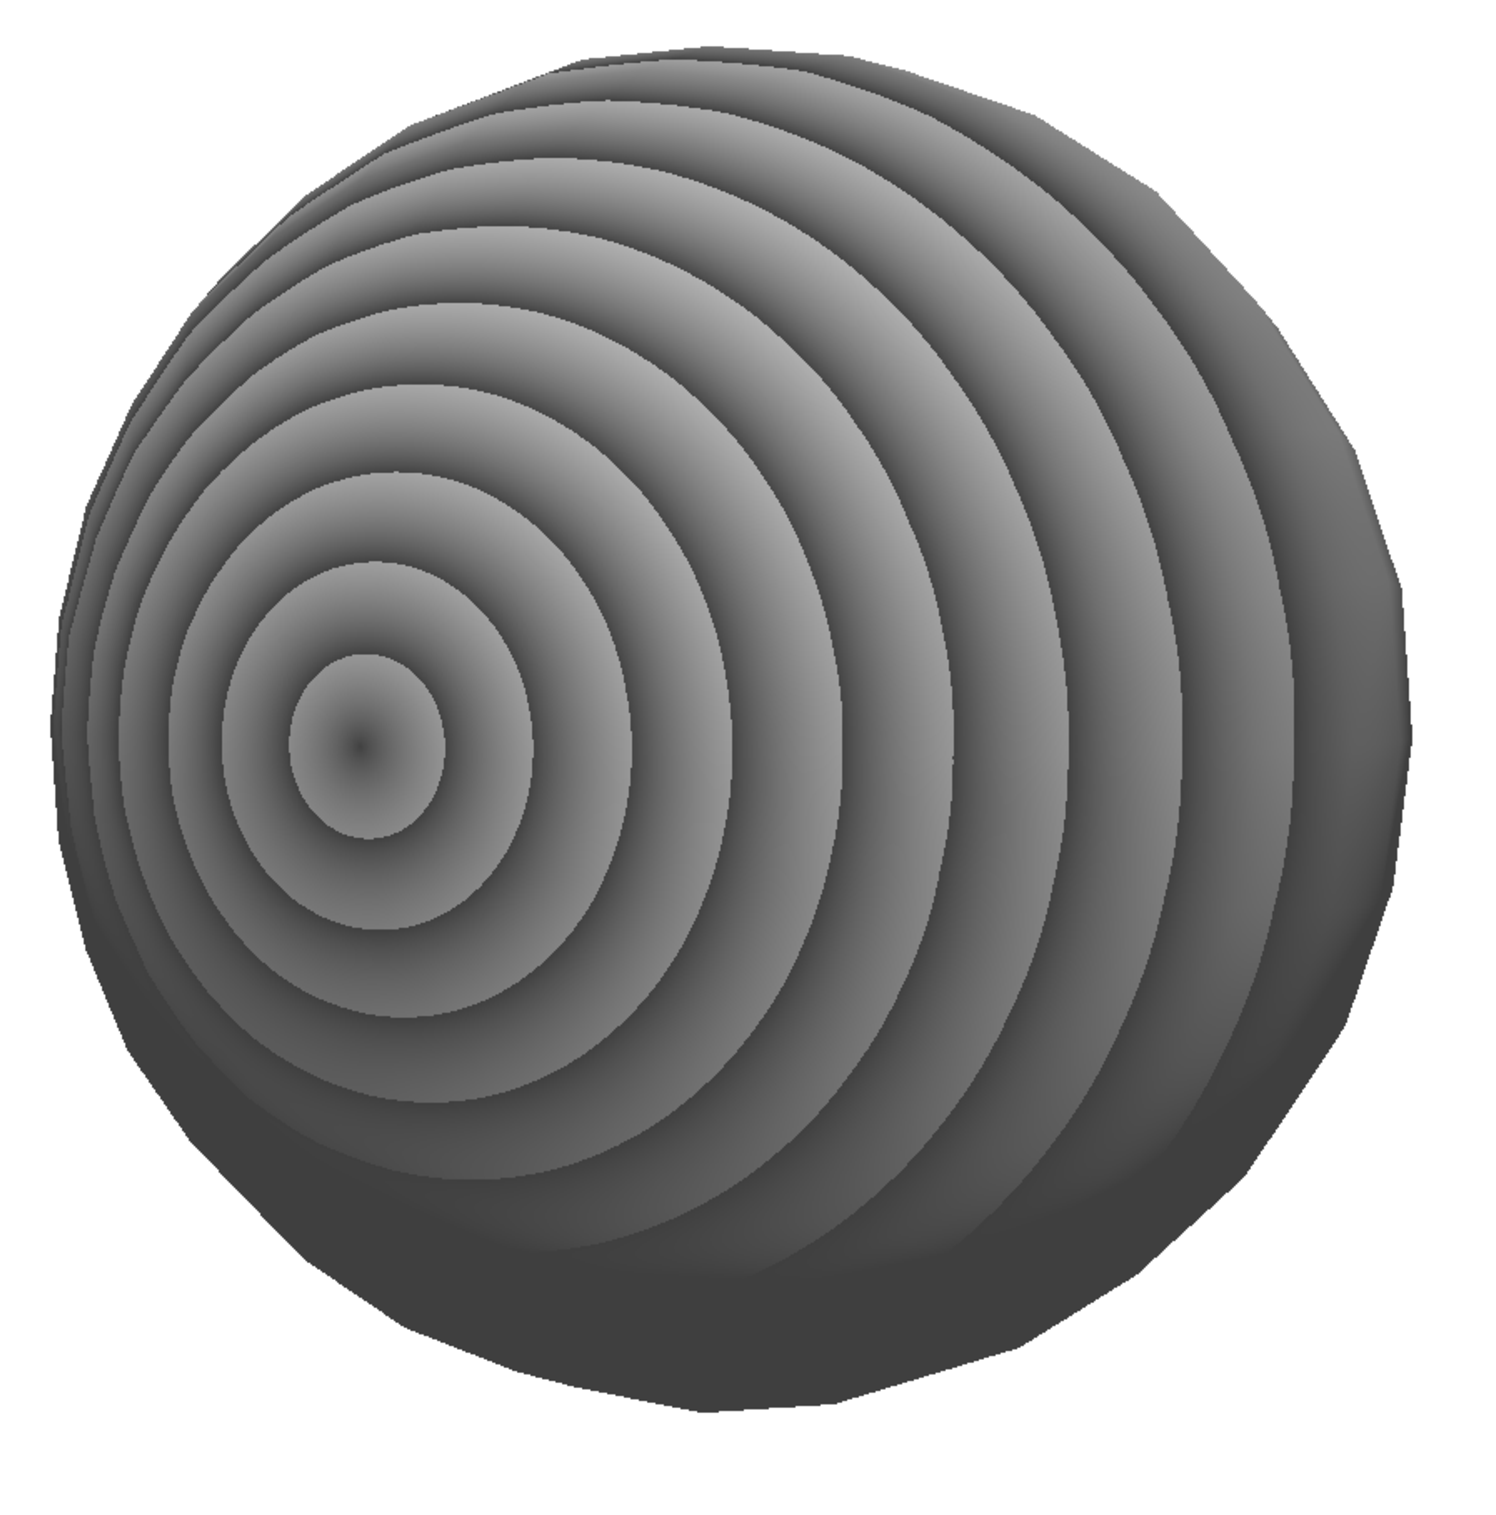
\includegraphics[width=.2\textwidth]{pics/procedural/letokruhy.eps}
\begin{minted}[bgcolor=bg]{packages/graphics.py:GLShaderLexer -x}
float d = length(model_pos.xy);
float t = mod(d*10, 1);
\end{minted}
\end{frame}

\begin{frame}[fragile]\frametitle{Coloring of annual rings / Letokruhy obarvíme}
  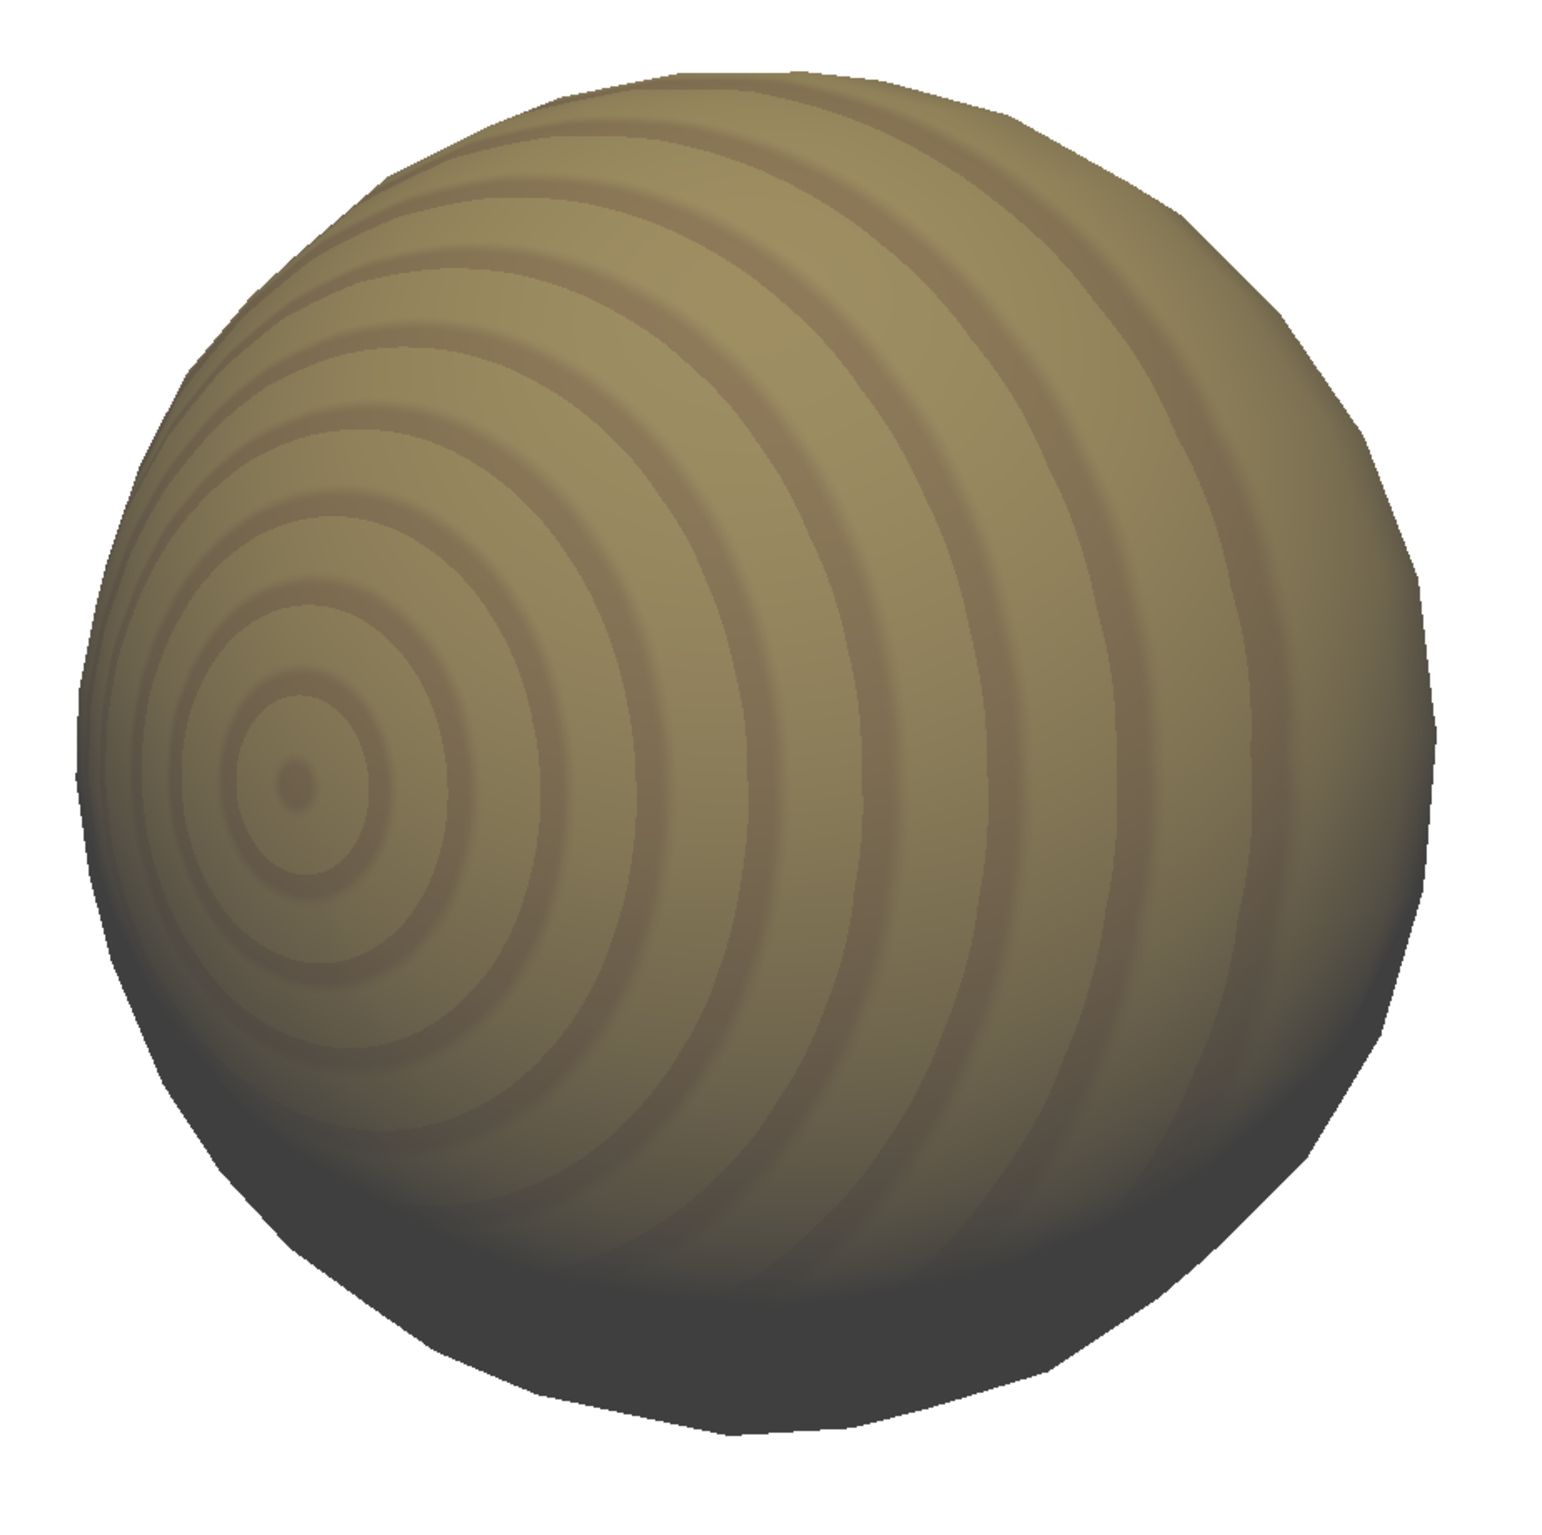
\includegraphics[width=.2\textwidth]{pics/procedural/letokruhy_barva.eps}
\begin{minted}[bgcolor=bg]{packages/graphics.py:GLShaderLexer -x}
vec3 brown = vec3(140, 90, 27)/255;
vec3 yellow = vec3(188, 140, 42)/255;

float t = smoothstep(0.2, 0.4, mod(length(model_pos.xy)*10, 1));
vec3 color = (1-t)*brown + t*yellow;
  \end{minted}
\end{frame}

\begin{frame}[fragile]\frametitle{Add turbulency with noise / Přidáme šum}
  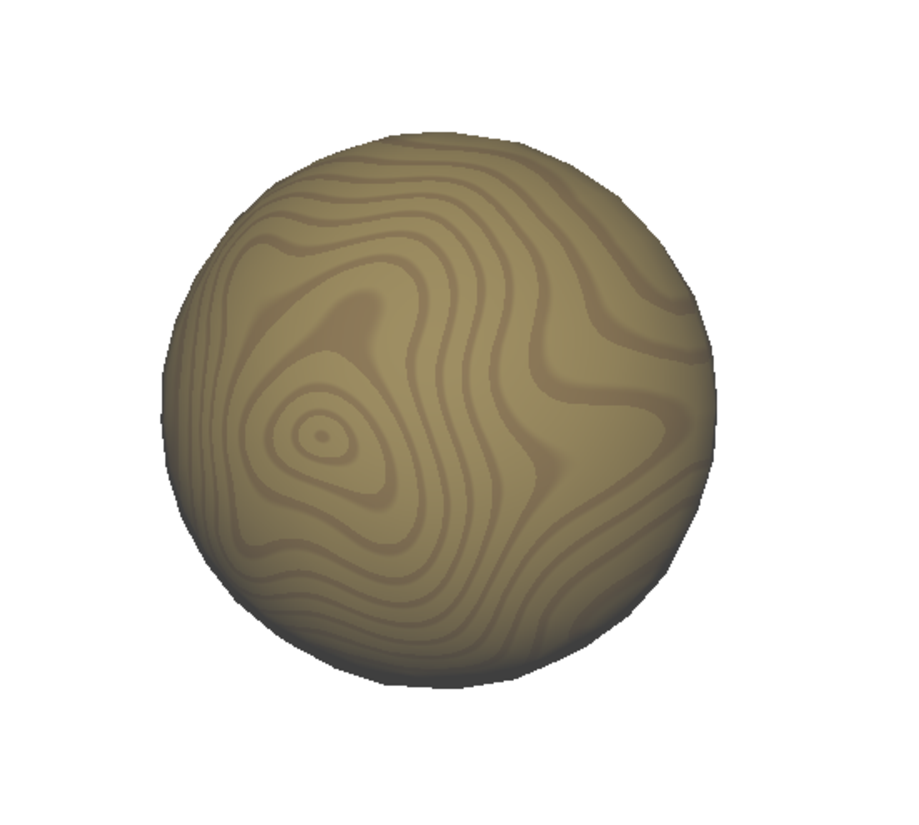
\includegraphics[width=.3\textwidth]{pics/procedural/drevo.eps}

\begin{minted}[bgcolor=bg]{packages/graphics.py:GLShaderLexer -x}
vec2 noisy_pos = model_pos.xy
    + 0.1*fnoise(model_pos.xy);

float t = smoothstep(0.2, 0.4, mod(length(noisy_pos)*10, 1));
vec3 color = (1-t)*brown + t*yellow;
  \end{minted}
\end{frame}

